\documentclass[10pt]{article}
\usepackage[utf8]{inputenc}
\usepackage{amsmath}
\usepackage{url}
\usepackage{hyperref}
\usepackage{listings}
\usepackage{microtype}
\usepackage{xcolor}
\usepackage{helvet} 
\usepackage{graphicx}
\usepackage{tikz}
\usepackage{multirow} 
\usepackage{wasysym}
\usepackage{rotating}
\usepackage{wrapfig}


\usepackage{tikz}
\usetikzlibrary{snakes,arrows,shapes}
\renewcommand{\familydefault}{\sfdefault}

\lstdefinelanguage{JavaScript}{
  keywords={typeof, new, true, false, catch, function, return, null, catch, switch, var, if, in, while, do, else, case, break},
  keywordstyle=\color{blue}\bfseries,
  ndkeywords={class, export, boolean, throw, implements, import, this},
  ndkeywordstyle=\color{darkgray}\bfseries,
  identifierstyle=\color{black},
  sensitive=false,
  comment=[l]{//},
  morecomment=[s]{/*}{*/},
  commentstyle=\color{purple}\ttfamily,
  stringstyle=\color{red}\ttfamily,
  morestring=[b]',
  morestring=[b]"
}



\newcommand{\jslisting}{   \lstset{
	language=JavaScript,
	emphstyle=\textbf,
	stringstyle=\texttt, 
	aboveskip=10pt,
	belowskip=10pt, 
	linewidth=\columnwidth,
	breaklines=true,
	basicstyle=\ttfamily,
	frame=single, 
	numbers=left,
	columns=flexible,
	showspaces=false,
	showstringspaces=false,
	moredelim=[is][\textbf]{|}{|}
   }}

\title{diretto API v1 Documentation}
%\subtitle{fobar}
\author{Benjamin Erb, Christian Koch, Stefan Kaufmann}
\date{September 2010}
\begin{document}

\maketitle

\subsection*{License}
\begin{figure}[!ht]
\begin{center}

\includegraphics[width=0.4\textwidth]{symbols/cc-By-nc-sa}
\end{center}
\end{figure}
This work is licensed under a Creative Commons Attribution-NonCommercial-
ShareAlike 3.0 License.

Symbols by Melih Bilgil (picol.org), Luka Pensa (pictoico.com), P.J. Onori
(somerandomdude.com) and Benjamin Erb.


\setcounter{tocdepth}{1}
\tableofcontents


\section{The API} % (fold)
\label{sec:doc_arc_API}

The API is the core of the whole diretto platform. It describes the external resource-oriented interfaces that clients and servers must implement. We tried to keep the API as simple as possbile while still laying the foundation for sophisticated usage. In this section, we first have a look at abstract composition of the API, followed by some technical details.

\subsection{Overview}
The API can be devided in to several interrelated resources:

\subsubsection{User}
\begin{wrapfigure}[4]{l}{0.06\textwidth}

\includegraphics[width=0.05\textwidth]{symbols/user_half.pdf}
\end{wrapfigure}
Most of the API calls require authentication. Each participant needs a valid user session, not matter if he is a human user or some kind of bot that executes tasks automatically. The current user model is flat, which means that there are no user hierarchies and each user has the same rights than all others. There are minor expcetions when it comes to user profiles or deletion of content. A user is currently identified by his registration e-mail address and personal password. Users can also choose an alias /user name, which does not have to be unique and is primarily for displaying users.


\subsubsection{Document}
\begin{wrapfigure}[4]{l}{0.06\textwidth}

\includegraphics[width=0.05\textwidth]{symbols/document_generic.pdf}
\end{wrapfigure}
 A document is a central entity in the diretto platform. Surprisingly, our documents do not represent distinct documents first-hand. Instead, they are abstract entities that group one or more concrete versions of the real document. This allows us the organize an original document and all its processed variants together. Also most of the meta data belong to the conceptual document rather than to distinct versions. A document belongs to a certain type of media, e.g. image.  

\subsubsection{Attachment} 
\begin{wrapfigure}[4]{l}{0.06\textwidth}

\includegraphics[width=0.05\textwidth]{symbols/attachment_add.pdf}
\end{wrapfigure}
Each document has one more associated attachment, whereas the first attachment always represents the original version. An attachment is a concrete media document that can be stored as a file and has a distinct mime type. Users can add new attachments to a document. Added variants should be derived or processed versions of the original attachment and should not add unrelated content.

\subsubsection{Tempo-Spatial Meta Data} 
\begin{wrapfigure}[4]{l}{0.06\textwidth}

\includegraphics[width=0.05\textwidth]{symbols/symbol_change_location.pdf}
\end{wrapfigure}
Every document has some kind of origin that is bound to a specific point in time and a location. If the document itself has a temporal duration, the point in time always refers to the beginning of the creation. Our platform can handle inaccurate data, which means that also spatial areas or time ranges can be indicated. Temporal and spatial data are decoupled so that the Cartesian product of all potential temporal and spatial data lists all potential origins of the document. A user can either suggest a new moment and/or location for a document, or he can vote for existing entries. 

\subsubsection{Link} 
\begin{wrapfigure}[4]{l}{0.06\textwidth}

\includegraphics[width=0.05\textwidth]{symbols/symbol_categories.pdf}
\end{wrapfigure}
Interconnections among documents can be specified as links. Such links represent semantical meanings between documents, such as cause-and-effect connections. Like doucments, links can be enriched with tags or key-value pairs. \newline


\subsubsection{Tag} 
\begin{wrapfigure}[4]{l}{0.06\textwidth}

\includegraphics[width=0.05\textwidth]{symbols/symbol_tag.pdf}
\end{wrapfigure}
Each attachment can be annotated with a tag. The tags in our platform are weighted, thus users can up-vote or down-vote tags. Tags enable users to collaboratively build taxonomies for the documents. \newline

\subsubsection{Comment} 
\begin{wrapfigure}[4]{l}{0.06\textwidth}

\includegraphics[width=0.05\textwidth]{symbols/symbol_comment.pdf}
\end{wrapfigure}
A attachment can be commented by a user with a text message. This allows an exchange of thoughts between the different users or even between the author and the viewers. \newline

\subsubsection{Key-Value Pair} 
\begin{wrapfigure}[4]{l}{0.06\textwidth}

\includegraphics[width=0.05\textwidth]{symbols/combine.pdf}
\end{wrapfigure}
While all other types of user-generated content mostly focus on humans, key-value pairs provide a type also for machine-based consumption. Each user has its own namespace where he can store simple text values under a given key name mapped to an attachment. These values can be read by all other users. Thanks to the user-separated namespaces, users can use the same keys concurrently --- values are still separated. Key-value pairs are helpful for annotating attachments with structural content that can be processed by bots or applications.

\subsubsection{Voting} 
\begin{wrapfigure}[4]{l}{0.06\textwidth}

\includegraphics[width=0.05\textwidth]{symbols/symbol_voting.pdf}
\end{wrapfigure}
Most of the user-generated content can be rated with an up-vote/down-vote. With an up-vote the user agrees that the entry is useful, valid or advantageous. Down-votes can be used to filter out incorrect or invalid entries. Voting can be applied to attachments, links, tags, comments and tempo-spatial meta data.


\subsection{Media Types}
The platform is not limited to images or other distinct media types. Basically, every possible type of media document can be used. Therefore, we only store very generic meta data about each entry directly. Detailed and specific meta data, like the resolution of an image or the duration of a video can still be saved as a key-value entry to the document. In order to make handling of different media types simple, we setup a threefold classification. Different traits of media objects can be used to group certain media object classes. Each usable media type must now be listed with its mime type and attached to one of the classes. 
This allows 
\begin{figure}[!ht]
\begin{center}
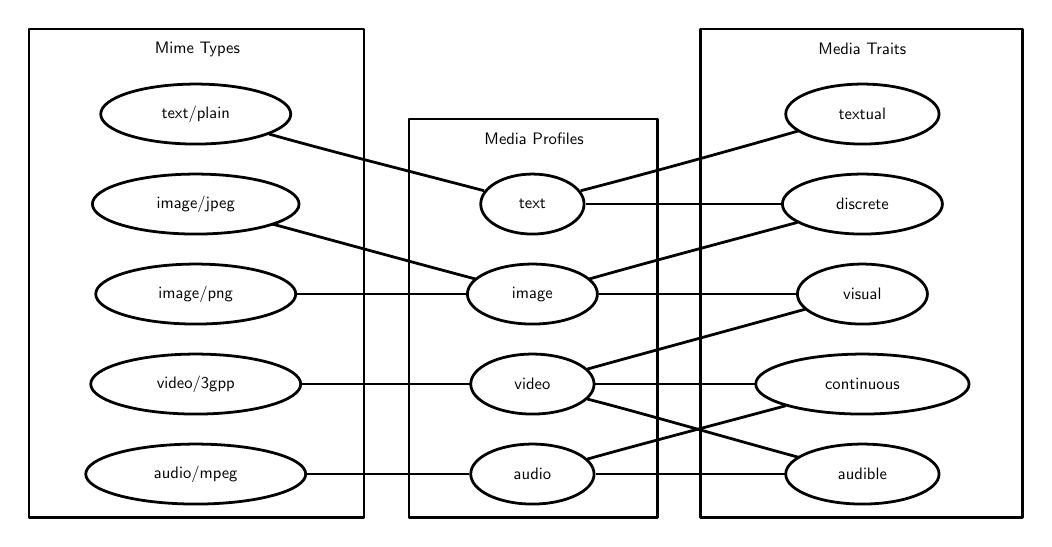
\begin{tikzpicture}[>=latex',line join=bevel,scale=0.6, transform shape]
  \pgfsetlinewidth{1bp}
%%
\begin{scope}
  \pgfsetstrokecolor{black}
  \draw (11bp,16bp) -- (11bp,309bp) -- (212bp,309bp) -- (212bp,16bp) -- cycle;
  \draw (112bp,297bp) node {Mime Types};
\end{scope}
\begin{scope}
  \pgfsetstrokecolor{black}
  \draw (239bp,16bp) -- (239bp,255bp) -- (388bp,255bp) -- (388bp,16bp) -- cycle;
  \draw (314bp,243bp) node {Media Profiles};
\end{scope}
\begin{scope}
  \pgfsetstrokecolor{black}
  \draw (414bp,16bp) -- (414bp,309bp) -- (607bp,309bp) -- (607bp,16bp) -- cycle;
  \draw (511bp,297bp) node {Media Traits};
\end{scope}
  \pgfsetcolor{black}
  % Edge: mime_png -- image
  \draw [] (172bp,150bp) .. controls (205bp,150bp) and (245bp,150bp)  .. (273bp,150bp);
  % Edge: mime_3gpp -- video
  \draw [] (174bp,96bp) .. controls (207bp,96bp) and (247bp,96bp)  .. (276bp,96bp);
  % Edge: text -- textual
  \draw [] (342bp,212bp) .. controls (377bp,221bp) and (435bp,237bp)  .. (473bp,248bp);
  % Edge: mime_jpeg -- image
  \draw [] (157bp,192bp) .. controls (194bp,182bp) and (245bp,168bp)  .. (279bp,159bp);
  % Edge: image -- discrete
  \draw [] (347bp,159bp) .. controls (382bp,169bp) and (435bp,183bp)  .. (472bp,193bp);
  % Edge: video -- continuous
  \draw [] (350bp,96bp) .. controls (377bp,96bp) and (415bp,96bp)  .. (447bp,96bp);
  % Edge: image -- visual
  \draw [] (353bp,150bp) .. controls (387bp,150bp) and (437bp,150bp)  .. (472bp,150bp);
  % Edge: video -- audible
  \draw [] (346bp,87bp) .. controls (381bp,78bp) and (436bp,62bp)  .. (473bp,52bp);
  % Edge: mime_mp3 -- audio
  \draw [] (178bp,42bp) .. controls (210bp,42bp) and (248bp,42bp)  .. (275bp,42bp);
  % Edge: mime_plain -- text
  \draw [] (155bp,246bp) .. controls (194bp,235bp) and (250bp,221bp)  .. (284bp,212bp);
  % Edge: video -- visual
  \draw [] (346bp,105bp) .. controls (382bp,115bp) and (441bp,131bp)  .. (477bp,141bp);
  % Edge: audio -- audible
  \draw [] (351bp,42bp) .. controls (383bp,42bp) and (430bp,42bp)  .. (465bp,42bp);
  % Edge: audio -- continuous
  \draw [] (346bp,51bp) .. controls (378bp,60bp) and (428bp,73bp)  .. (465bp,83bp);
  % Edge: text -- discrete
  \draw [] (345bp,204bp) .. controls (377bp,204bp) and (426bp,204bp)  .. (462bp,204bp);
  % Node: continuous
\begin{scope}
  \pgfsetstrokecolor{black}
  \draw (511bp,96bp) ellipse (64bp and 18bp);
  \draw (511bp,96bp) node {continuous};
\end{scope}
  % Node: mime_png
\begin{scope}
  \pgfsetstrokecolor{black}
  \draw (111bp,150bp) ellipse (60bp and 18bp);
  \draw (111bp,150bp) node {image/png};
\end{scope}
  % Node: text
\begin{scope}
  \pgfsetstrokecolor{black}
  \draw (313bp,204bp) ellipse (31bp and 18bp);
  \draw (313bp,204bp) node {text};
\end{scope}
  % Node: image
\begin{scope}
  \pgfsetstrokecolor{black}
  \draw (313bp,150bp) ellipse (39bp and 18bp);
  \draw (313bp,150bp) node {image};
\end{scope}
  % Node: mime_mp3
\begin{scope}
  \pgfsetstrokecolor{black}
  \draw (111bp,42bp) ellipse (66bp and 18bp);
  \draw (111bp,42bp) node {audio/mpeg};
\end{scope}
  % Node: mime_3gpp
\begin{scope}
  \pgfsetstrokecolor{black}
  \draw (111bp,96bp) ellipse (63bp and 18bp);
  \draw (111bp,96bp) node {video/3gpp};
\end{scope}
  % Node: textual
\begin{scope}
  \pgfsetstrokecolor{black}
  \draw (511bp,258bp) ellipse (46bp and 18bp);
  \draw (511bp,258bp) node {textual};
\end{scope}
  % Node: mime_plain
\begin{scope}
  \pgfsetstrokecolor{black}
  \draw (111bp,258bp) ellipse (57bp and 18bp);
  \draw (111bp,258bp) node {text/plain};
\end{scope}
  % Node: mime_jpeg
\begin{scope}
  \pgfsetstrokecolor{black}
  \draw (111bp,204bp) ellipse (62bp and 18bp);
  \draw (111bp,204bp) node {image/jpeg};
\end{scope}
  % Node: discrete
\begin{scope}
  \pgfsetstrokecolor{black}
  \draw (511bp,204bp) ellipse (48bp and 18bp);
  \draw (511bp,204bp) node {discrete};
\end{scope}
  % Node: visual
\begin{scope}
  \pgfsetstrokecolor{black}
  \draw (511bp,150bp) ellipse (39bp and 18bp);
  \draw (511bp,150bp) node {visual};
\end{scope}
  % Node: video
\begin{scope}
  \pgfsetstrokecolor{black}
  \draw (313bp,96bp) ellipse (37bp and 18bp);
  \draw (313bp,96bp) node {video};
\end{scope}
  % Node: audio
\begin{scope}
  \pgfsetstrokecolor{black}
  \draw (313bp,42bp) ellipse (37bp and 18bp);
  \draw (313bp,42bp) node {audio};
\end{scope}
  % Node: audible
\begin{scope}
  \pgfsetstrokecolor{black}
  \draw (511bp,42bp) ellipse (46bp and 18bp);
  \draw (511bp,42bp) node {audible};
\end{scope}
%
\end{tikzpicture}
\caption{Threefold classification of different media types}
\label{medtypes}
\end{center}
\end{figure}

This classification allows an abstract view onto the different media objects. It allows clients to implement features based upon the media traits or media class profiles instead of concrete mime types, which makes the clients more versatile.



\section{Guidelines for the API documentation}
\label{sec:app_api_intro}

This documentation represents a technical documentation of our RESTful API. It is the primary source of information for implementing own client or server applications without using existing libraries. Each logical API action is mapped to a distinct HTTP request and described in detail. The following characteristics are used therefore:

\begin{description}

	\item[URI] The URI against the API call must be invoked. It may contain placeholders and parameters that are described below. In order to provide flexibility with future versions of the API, the APIs are versioned by adding a version parameter to the path. So for the current version, the string "v1" must be appended to the server API root path, resulting in http://apipath/v1. 

	\item[HTTP Methods] Lists the valid HTTP mehtod(s) that can be used to invoke this API call.

	\item[Parameters] Lists all URI parameters and their allowed values. 

	\item[Formats] The valid data formats that can be used in this API call for entities.

	\item[Authentication Required] Stats whether an authentication is required for this API call or not. Most of the API methods do need authentication.

	\item[Request Entity] If a request contains an entity body, an exemplary entity is shown.

	\item[Responses] Lists all HTTP response codes and their concrete meaning for this API call. Note that there are other repsonse codes that can be received on every request, like a \texttt{500} for an generic server-side error. The response codes listed in the an API call documentation are the codes specific for the current request.

	\item[Response Entity]  If a request contains an entity body, an exemplary entity is shown. If an error occurs, there is always a simple JSON object struct with the key \texttt{error} that contains a textual error message as its respective value.

\end{description}

\section{Attachments}
The following actions provide methods related to the document attachments and their meta data.

\subsection{Get an attachment }
Returns metadata of the attachment.
\subsubsection{URI}
\texttt{http://apipath/documents/\fbox{doc-id}/attachments/\fbox{attachment-id}
}
\subsubsection{HTTP Methods}
\texttt{GET}
\subsubsection{Parameters}
\begin{tabular}{|l|l|}\hline
doc-id & UUID of the document \\
\hline
attachment-id & UUID of the attachment \\
\hline
\end{tabular}
\subsubsection{Formats}
JSON
\subsubsection{Authentication Required}
true
\subsubsection{Request Entity}
n/a
\subsubsection{Responses}
\begin{tabular}{|l|l|}\hline
200 & Attachment metadata in body \\
\hline
202 & Attachment known, but upload pending \\
\hline
404 & Attachment not found \\
\hline
\end{tabular}
\subsubsection{Response Entity}

\jslisting
\lstset{caption=}
\begin{lstlisting}
{
   "attachmentId":"e5fba1fd-0717-4197-a40a-b2a5e079f715",
   "docId":"e5fba1fd-0717-4197-a40a-b2a5e079f715",
   "mimetype":"text/plain",
   "size":1064,
   "uploader":"foo",
   "uploaded":"2010-07-17T18:54:11.947Z",
   "location":"http://api.diretto.org:8000/e5fba1fd-0717-4197-a40a-b2a5e079f715/e5fba1fd-0717-4197-a40a-b2a5e079f715.txt"
}
\end{lstlisting}

\subsection{Get the list of attachment IDs for a document }
Returns metadata of the document
\subsubsection{URI}
\texttt{http://apipath/documents/\fbox{doc-id}/attachments
}
\subsubsection{HTTP Methods}
\texttt{GET}
\subsubsection{Parameters}
\begin{tabular}{|l|l|}\hline
doc-id & UUID of the document \\
\hline
\end{tabular}
\subsubsection{Formats}
JSON
\subsubsection{Authentication Required}
true
\subsubsection{Request Entity}
n/a
\subsubsection{Responses}
\begin{tabular}{|l|l|}\hline
200 & Attachment id list in body \\
\hline
404 & Document not found \\
\hline
\end{tabular}
\subsubsection{Response Entity}
\jslisting
\lstset{caption=}
\begin{lstlisting}
{
   "documentId":"e5fba1fd-0717-4197-a40a-b2a5e079f715",
   "attachmentIds":[
      "e5fba1fd-0717-4197-a40a-b2a5e079f715",
      "550e8400-e29b-11d4-a716-446655440000"
   ]
}
\end{lstlisting}



\subsection{Forward from alias URI}
Forwards the alias URI without document id to the correct URI including document.
\subsubsection{URI}
\texttt{http://apipath/attachments/\fbox{attach-id}
}
\subsubsection{HTTP Methods}
\texttt{GET}
\subsubsection{Parameters}
\begin{tabular}{|l|l|}\hline
attach-id & Attachment ID \\
\hline
\end{tabular}
\subsubsection{Formats}
n/a
\subsubsection{Authentication Required}
true
\subsubsection{Request Entity}
n/a
\subsubsection{Responses}
\begin{tabular}{|l|l|}\hline
303 See Other + Location  & Forward to correct URI \\
\hline
404 Not found & Attachment not found \\
\hline
\end{tabular}
\subsubsection{Response Entity}
n/a


\subsection{List all attachements}
Lists the id and mime type of all uploaded documents sorted by upload time. Results are split up into chunks of 100 documents. Navigation within the pagination is possible using cursor ids. These ids represent the first entry of a chunk of the previous/following result page. First/last page omits the previous/next key-value pair. A request without cursor will start with the first available value as cursor.
\subsubsection{URI}
\begin{itemize}
\item \texttt{http://apipath/attachments/\fbox{ascending|descending}/ }=> will be 303'ed  to \texttt{http://apipath/attachments/\fbox{ascending|descending}/cursor/\fbox{firstcursor}
}
\item \texttt{http://apipath/attachments/\fbox{ascending|descending}/cursor/\fbox{documentid}
}
\end{itemize}
\subsubsection{HTTP Methods}
\texttt{GET}
\subsubsection{Parameters}
n/a
\subsubsection{Formats}
JSON
\subsubsection{Authentication Required}
true
\subsubsection{Request Entity}
n/a
\subsubsection{Responses}
\begin{tabular}{|l|l|}\hline
200 Accepted & List delivered \\
\hline
303 See Other + Location including first cursor & Query without cursor \\
\hline
404 Not found & Cursor not found \\
\hline
\end{tabular}

\subsubsection{Response Entity}
\jslisting
\lstset{caption=}
\begin{lstlisting}
{
  "attachments" : [
    {"id" : "3e64c371ba2b93f1c0fead369fe004ef", "mimetype" : "image/jpeg" },
    //98 other entries here...
    {"id" : "57ebb75106e99f6e7299fefe37de83b7", "mimetype" : "text/plain" }
  ],
  "next" : "acbd18db4cc2f85cedef654fccc4a4d8",
  "previous" : "37b51d194a7513e45b56f6524f2d51f2",
  "total" : 1234
}
\end{lstlisting}

\section{Comments}
\subsection{Commentable Items}
Comments can be added to the following items:
\begin{itemize}
 \item Attachments
   \item base URI = \texttt{\texttt{http://apipath/documents/\fbox{doc-id}/attachments/\fbox{attachment-id}}
} \item Links
   \item base URI = \texttt{\texttt{http://apipath/links/\fbox{link-id}} }
\end{itemize}
\subsection{List comments by attachment}
Returns a list of comments of a attachment.
\subsubsection{URI}
\texttt{http://apipath/documents/\fbox{doc-id}/attachments/\fbox{attachment-id}/comments
}\subsubsection{HTTP Methods}
\texttt{GET}
\subsubsection{Parameters}
\begin{tabular}{|l|l|}\hline
doc-id & UUID of the document \\
\hline
attachment-id & UUID of the attachment \\
\hline
\end{tabular}
\subsubsection{Formats}
JSON
\subsubsection{Authentication Required}
true
\subsubsection{Request Entity}
n/a
\subsubsection{Responses}
\begin{tabular}{|l|l|}\hline
200 & List of comments \\
\hline
404 & Document/Attachment not found \\
\hline
\end{tabular}
\subsubsection{Response Entity}
\jslisting
\lstset{caption=}
\begin{lstlisting}
{
   "comments":[
      {
         "comment_id":"d4777513-7eb6-de3d-6c90-81cd8205c376",
         "doc_id":"e08eee5b-ba09-484a-b25d-1b7f2b7ae45c",
         "attachment_id":"e08eee5b-ba09-484a-b25d-1b7f2b7ae45c",
         "user":"foox",
         "comment":"blablabla",
         "created":"2010-09-02T14:22:13.744Z"
      },
      {
         "comment_id":"ffb4480c-5a9a-481a-821a-b4b3c0c917d0",
         "doc_id":"e08eee5b-ba09-484a-b25d-1b7f2b7ae45c",
         "attachment_id":"e08eee5b-ba09-484a-b25d-1b7f2b7ae45c",
         "user":"foox",
         "comment":"blablabla2",
         "created":"2010-09-02T14:22:13.844Z"
      }
   ],
   "total":2
}
\end{lstlisting}
\subsection{Get a attachment comment by comment ID}
Returns a comment by ID. Alternatively, you can query \texttt{http://apipath/comments/\fbox{comment-id} }and will be 303'ed to the right URL with document and attachment ID.
\subsubsection{URI}
\texttt{http://apipath/documents/\fbox{doc-id}/attachments/\fbox{attachment-id}/comments/\fbox{comment-id}
}\texttt{http://apipath/comments/\fbox{comment-id} }(see description above)
\subsubsection{HTTP Methods}
\texttt{GET}
\subsubsection{Parameters}
\begin{tabular}{|l|l|}\hline
doc-id & UUID of the document \\
\hline
attachment-id & UUID of the attachment \\
\hline
comment-id & UUID of the comment \\
\hline
\end{tabular}
\subsubsection{Formats}
JSON
\subsubsection{Authentication Required}
true
\subsubsection{Request Entity}
n/a
\subsubsection{Responses}
\begin{tabular}{|l|l|}\hline
200 & Comment \\
\hline
404 & Comment not found \\
\hline
\end{tabular}
\subsubsection{Response Entity}
\jslisting
\lstset{caption=}
\begin{lstlisting}
{
   "comment_id":"d4777513-7eb6-de3d-6c90-81cd8205c376",
   "doc_id":"e08eee5b-ba09-484a-b25d-1b7f2b7ae45c",
   "attachment_id":"e08eee5b-ba09-484a-b25d-1b7f2b7ae45c",
   "created":"2010-09-02T14:22:13.744Z",
   "type":"comment",
   "user":"foox",
   "comment":"blablabla"
}
\end{lstlisting}
\subsection{Create a new comment for an attachment}
Post a new comment to the given attachment.
\subsubsection{URI}
\texttt{http://apipath/documents/\fbox{doc-id}/attachments/\fbox{attachment-id}/comments
}\subsubsection{HTTP Methods}
\texttt{POST}
\subsubsection{Parameters}
\begin{tabular}{|l|l|}\hline
doc-id & UUID of the document \\
\hline
attachment-id & UUID of the attachment \\
\hline
\end{tabular}
\subsubsection{Formats}
JSON
\subsubsection{Authentication Required}
true
\subsubsection{Request Entity}
\jslisting
\lstset{caption=}
\begin{lstlisting}
{
   "comment":"blablabla"
}
\end{lstlisting}
\subsubsection{Responses}
\begin{tabular}{|l|l|}\hline
201 & List of comments \\
\hline
400 & Invalid comment data \\
\hline
404 & Document/Attachment not found \\
\hline
\end{tabular}
\subsubsection{Response Entity}
n/a
\subsection{List attachment comments by user}
Returns a list of comments by user
\subsubsection{URI}
\texttt{http://apipath/users/\fbox{user-id}/comments
}\subsubsection{HTTP Methods}
\texttt{GET}
\subsubsection{Parameters}
\begin{tabular}{|l|l|}\hline
user-id & The ID of the user \\
\hline
\end{tabular}
\subsubsection{Formats}
JSON
\subsubsection{Authentication Required}
true
\subsubsection{Request Entity}
n/a
\subsubsection{Responses}
\begin{tabular}{|l|l|}\hline
200 & List of comments \\
\hline
404 & user not found \\
\hline
\end{tabular}
\subsubsection{Response Entity}
\jslisting
\lstset{caption=}
\begin{lstlisting}
{
   "comments":[
      {
         "comment_id":"d4777513-7eb6-de3d-6c90-81cd8205c376",
         "doc_id":"e08eee5b-ba09-484a-b25d-1b7f2b7ae45c",
         "attachment_id":"e08eee5b-ba09-484a-b25d-1b7f2b7ae45c",
         "user":"foox",
         "comment":"blablabla",
         "created":"2010-09-02T14:22:13.744Z"
      }     
   ],
   "total":1
}
\end{lstlisting}
\subsection{List comments by link}
Returns a list of comments of a link.
\subsubsection{URI}
\texttt{http://apipath/links/\fbox{link-id}/comments
}\subsubsection{HTTP Methods}
\texttt{GET}
\subsubsection{Parameters}
\begin{tabular}{|l|l|}\hline
link-id & UUID of the link \\
\hline
\end{tabular}
\subsubsection{Formats}
JSON
\subsubsection{Authentication Required}
true
\subsubsection{Request Entity}
n/a
\subsubsection{Responses}
\begin{tabular}{|l|l|}\hline
200 & List of comments \\
\hline
404 & Link not found \\
\hline
\end{tabular}
\subsubsection{Response Entity}
\jslisting
\lstset{caption=}
\begin{lstlisting}
{
   "comments":[
      {
         "comment_id":"d4777513-7eb6-de3d-6c90-81cd8222b846",
         "link_id":"d4777513-7eb6-de3d-6c90-81cd82215410",
         "user":"foox",
         "comment":"bla",
         "created":"2010-09-12T19:17:46.344Z"
      },
      {
         "comment_id":"d4777513-7eb6-de3d-6c90-81cd8222c1e1",
         "link_id":"d4777513-7eb6-de3d-6c90-81cd82215410",
         "user":"foox",
         "comment":"bla",
         "created":"2010-09-12T19:18:02.334Z"
      }
   ],
   "total":2
}
\end{lstlisting}
\subsection{Get a link comment by comment ID}
Returns a comment by ID. Alternatively, you can query \texttt{http://apipath/comments/\fbox{comment-id} }and will be 303'ed to the right URL with document and attachment ID.
\subsubsection{URI}
\texttt{http://apipath/links/\fbox{link-id}/comments/\fbox{comment-id}
}\texttt{http://apipath/comments/\fbox{comment-id} }(see description above)
\subsubsection{HTTP Methods}
\texttt{GET}
\subsubsection{Parameters}
\begin{tabular}{|l|l|}\hline
link-id & UUID of the link \\
\hline
comment-id & UUID of the comment \\
\hline
\end{tabular}
\subsubsection{Formats}
JSON
\subsubsection{Authentication Required}
true
\subsubsection{Request Entity}
n/a
\subsubsection{Responses}
\begin{tabular}{|l|l|}\hline
200 & Comment \\
\hline
404 & Comment not found \\
\hline
\end{tabular}
\subsubsection{Response Entity}
\jslisting
\lstset{caption=}
\begin{lstlisting}
{
   "comment_id":"d4777513-7eb6-de3d-6c90-81cd8222c1e1",
   "link_id":"d4777513-7eb6-de3d-6c90-81cd82215410",
   "created":"2010-09-12T19:18:02.334Z",
   "type":"comment",
   "user":"foox",
   "comment":"bla"
}
\end{lstlisting}
\subsection{Create a new comment for a link}
Post a new comment to the given link.
\subsubsection{URI}
\texttt{http://apipath/links/\fbox{link-id}/comments
}\subsubsection{HTTP Methods}
\texttt{POST}
\subsubsection{Parameters}
\begin{tabular}{|l|l|}\hline
link-id & UUID of the link \\
\hline
\end{tabular}
\subsubsection{Formats}
JSON
\subsubsection{Authentication Required}
true
\subsubsection{Request Entity}
\jslisting
\lstset{caption=}
\begin{lstlisting}
{
   "comment":"blablabla"
}
\end{lstlisting}
\subsubsection{Responses}
\begin{tabular}{|l|l|}\hline
201 & List of comments \\
\hline
400 & Invalid comment data \\
\hline
404 & Link not found \\
\hline
\end{tabular}
\subsubsection{Response Entity}
n/a
\section{Documents}
The following actions provide methods related to the documents collected by the users and their meta data.
[[TitleIndex(Components/API/v1/REST/Documents,format=group)]]
\subsection{Get a document }
Returns metadata of the document
\subsubsection{URI}
\texttt{http://apipath/documents/\fbox{doc-id}
}\subsubsection{HTTP Methods}
\texttt{GET}
\subsubsection{Parameters}
\begin{tabular}{|l|l|}\hline
doc-id & UUID of the new document \\
\hline
\end{tabular}
\subsubsection{Formats}
JSON
\subsubsection{Authentication Required}
true
\subsubsection{Request Entity}
n/a
\subsubsection{Responses}
\begin{tabular}{|l|l|}\hline
200 & Document metadata in body \\
\hline
202 & Document known, but upload pending \\
\hline
404 & Document not found \\
\hline
\end{tabular}
\subsubsection{Response Entity}
\jslisting
\lstset{caption=}
\begin{lstlisting}
{
  "id":"d16e103e-4fda-433d-9309-179487ecad4a",
  "mediatype":"text",
  "owner":"foo",
  "uploaded":"2010-07-17T18:54:11.939Z"
}
\end{lstlisting}
\subsection{Metadata upload for a new document }
Uploads metadata as an initial step for creating a new document.
\subsubsection{URI}
\texttt{http://apipath/documents/\fbox{doc-id}
}\subsubsection{HTTP Methods}
\texttt{PUT}
\subsubsection{Parameters}
\begin{tabular}{|l|l|}\hline
doc-id & UUID of the new document \\
\hline
\end{tabular}
\subsubsection{Formats}
JSON
\subsubsection{Authentication Required}
true
\subsubsection{Request Entity}
\texttt{PUT /v1/documents/d16e103e-4fda-433d-9309-179487ecad4a}
\jslisting
\lstset{caption=}
\begin{lstlisting}
{
   "document":{
      "date":{
         "before":"2010-06-29T19:15:51.765Z",
         "after":"2010-06-29T19:15:50.000Z"
      },
      "location":{
         "position":{
            "type":"Point",
            "coordinates":[
               100.0,
               0.0
            ]
         },
         "variance": 100
      }
   },
   "attachment":{
      "contentType":"image/jpeg",
      "contentLength":123
   }
}
\end{lstlisting}
\subsubsection{Responses}
\begin{tabular}{|l|l|}\hline
202 & Accepted + Entity \\
\hline
400 & Invalid metadata \\
\hline
409 & Document already exists \\
\hline
413 & Document content content is to large \\
\hline
415 & Document content type is not supported \\
\hline
\end{tabular}
\subsubsection{Response Entity}
\jslisting
\lstset{caption=}
\begin{lstlisting}
{
   "upload":{
      "key":"00b19c9d7db4f1ae0824c62bda5a127588bde476",
      "location":"http://localhost:8000/d16e103e-4fda-433d-9309-179487ecad4a/d16e103e-4fda-433d-9309-179487ecad4a.jpg",
      "uri":"http://localhost:8000/d16e103e-4fda-433d-9309-179487ecad4a/d16e103e-4fda-433d-9309-179487ecad4a.jpg?key=00b19c9d7db4f1ae0824c62bda5a127588bde476"
   }
}
\end{lstlisting}
\subsection{Confirm successful upload}
As last step of an upload process, the client must confirm the successful upload by releasing document lock.
\subsubsection{URI}
\texttt{http://apipath/documents/\fbox{doc-id}/attachments/\fbox{attach-id}/lock/\fbox{lock-id}
}\subsubsection{HTTP Methods}
\texttt{DELETE}
\subsubsection{Parameters}
\begin{tabular}{|l|l|}\hline
doc-id & UUID of the new document \\
\hline
attach-id & generated UUID of the attachment (equals doc-id in case of new attachments) \\
\hline
lock-id & Lock ID provided by the media node \\
\hline
\end{tabular}
\subsubsection{Formats}
n/a
\subsubsection{Authentication Required}
true
\subsubsection{Request Entity}
n/a
\subsubsection{Responses}
\begin{tabular}{|l|l|}\hline
204 & Upload completed \\
\hline
403 & Invalid lock release (lock id does not match/wrong user) \\
\hline
\end{tabular}
\subsubsection{Response Entity}
n/a
\subsection{List all documents}
Lists the id and type of all uploaded documents sorted by upload time. Results are split up into chunks of 100 documents. Navigation within the pagination is possible using cursor ids. These ids represent the first entry of a chunk of the previous/following result page. First/last page omits the previous/next key-value pair. A request without cursor will start with the first available value as cursor.
\subsubsection{URI}
\begin{itemize}
\item \texttt{http://apipath/documents/\fbox{ascending|descending}/ }=> will be 303'ed  to \texttt{http://apipath/documents/\fbox{ascending|descending}/cursor/\fbox{firstcursor}
}\item \texttt{http://apipath/documents/\fbox{ascending|descending}/cursor/\fbox{documentid}
}\end{itemize}
\subsubsection{HTTP Methods}
\texttt{GET}
\subsubsection{Parameters}
\begin{tabular}{|l|l|}\hline
order & ascending or descending \\
\hline
\end{tabular}
\subsubsection{Formats}
JSON
\subsubsection{Authentication Required}
true
\subsubsection{Request Entity}
n/a
\subsubsection{Responses}
\begin{tabular}{|l|l|}\hline
200 Accepted & List delivered \\
\hline
303 See Other + Location including first cursor & Query without cursor \\
\hline
404 Not found & Cursor not found \\
\hline
\end{tabular}
\subsubsection{Response Entity}
\jslisting
\lstset{caption=}
\begin{lstlisting}
{
  "documents" : [
    {"id" : "3e64c371ba2b93f1c0fead369fe004ef", "type" : "image" },
    //98 other entries here...
    {"id" : "57ebb75106e99f6e7299fefe37de83b7", "type" : "video" }
  ],
  "next" : "acbd18db4cc2f85cedef654fccc4a4d8",
  "previous" : "37b51d194a7513e45b56f6524f2d51f2",
  "total" : 1234
}
\end{lstlisting}
\subsection{List documents uploaded before or after a distinct point in time}
This method allows to scroll through document lists by a given point in time as cursor. It either moves chronologically (descending) to newer documents added after the time (after semantics) or ascending to older ones  (before semantics). If there is an exact match for the given time/date, this document will be used as resolved curosr, otherwise the next matching document in order will be. 
The time cursor must be a valid RFC 3339 timestamp like \texttt{2010-06-29T19:15:51.765Z}.
\subsubsection{URI}
\begin{itemize}
\item \texttt{http://apipath/documents/\fbox{before|after}/\fbox{date} }=> will be 303'ed  to \texttt{http://apipath/documents/\fbox{ascending|descending}/cursor/\fbox{firstcursor}
}\end{itemize}
\subsubsection{HTTP Methods}
\texttt{GET}
\subsubsection{Parameters}
\begin{tabular}{|l|l|}\hline
cursor type  &  before/after \\
\hline
date & Valid RFC 3339 timestamp used as split point  \\
\hline
\end{tabular}
\subsubsection{Formats}
n/a
\subsubsection{Authentication Required}
true
\subsubsection{Request Entity}
n/a
\subsubsection{Responses}
\begin{tabular}{|l|l|}\hline
204 Not found & No documents available \\
\hline
303 See Other + Location including first cursor & Query without cursor \\
\hline
404 Not found & Cursor not found \\
\hline
\end{tabular}
\subsubsection{Response Entity}
n/a
\section{Index}
This represents the root path of the diretto webservice.
\subsection{Get service root }
Returns information about the web service.
\subsubsection{URI}
\texttt{http://apipath
}\subsubsection{HTTP Methods}
\texttt{GET}
\subsubsection{Parameters}
n/a
\subsubsection{Formats}
JSON
\subsubsection{Authentication Required}
false
\subsubsection{Request Entity}
n/a
\subsubsection{Responses}
\begin{tabular}{|l|l|}\hline
200 OK & Response entity containing the info \\
\hline
\end{tabular}
\subsubsection{Response Entity}
\jslisting
\lstset{caption=}
\begin{lstlisting}
{
   "version":"v1",
   "deployment":{
      "title":"diretto Project Team Development ",
      "contact":"n/a",
      "website":"http://www.diretto.org"
   },
   "service":{
      "uri":"http://localhost:8001/"
   },
   "mediaserver":{
      "uri":"http://localhost:8000/"
   }
}
\end{lstlisting}
\section{KeyValues}
Users can add text-based key-value pairs to some entries. Each user has its own namespace, thus multiple users can use the same keys concurrently. A pair can only be created, modified and deleted by the user, but every other user has read-only access to it. So values should not be used for private or restricted information. Note that values must only be strings, so structured formats might need to be serialized first. A concrete service may also limit the amount of values per entry or the maximal size per value. 
\subsection{Types that can be labelled with a key-value pairs}
\begin{itemize}
 \item Attachments
   \item base URI = \texttt{\texttt{http://apipath/documents/\fbox{doc-id}/attachments/\fbox{attachment-id}}
} \item Links
   \item base URI = \texttt{\texttt{http://apipath/links/\fbox{link-id}} }
\end{itemize}
\subsection{Return a list of key/values of an attachment}
List all pairs of the given attachment.
\subsubsection{URI}
\texttt{http://apipath/documents/\fbox{doc-id}/attachments/\fbox{attachment-id}/values
}\subsubsection{HTTP Methods}
\texttt{GET}
\subsubsection{Parameters}
\begin{tabular}{|l|l|}\hline
doc-id & UUID of the document \\
\hline
attachment-id & UUID of the attachment \\
\hline
\end{tabular}
\subsubsection{Formats}
JSON
\subsubsection{Authentication Required}
true
\subsubsection{Request Entity}
n/a
\subsubsection{Responses}
\begin{tabular}{|l|l|}\hline
200 & OK \\
\hline
404 & Link not found \\
\hline
\end{tabular}
\subsubsection{Response Entity}
\jslisting
\lstset{caption=}
\begin{lstlisting}
{
   "values":[
      {
         "key":"foo",
         "user":"foox",
         "value":"bar",
      }
   ],
   "total":1
}
\end{lstlisting}
\subsection{Insert a new pair to an attchment}
Post a new pair to the given attachment.
\subsubsection{URI}
\texttt{http://apipath/documents/\fbox{doc-id}/attachments/\fbox{attachment-id}/values
}\subsubsection{HTTP Methods}
\texttt{POST}
\subsubsection{Parameters}
\begin{tabular}{|l|l|}\hline
doc-id & UUID of the document \\
\hline
attachment-id & UUID of the attachment \\
\hline
\end{tabular}
\subsubsection{Formats}
JSON
\subsubsection{Authentication Required}
true
\subsubsection{Request Entity}
\jslisting
\lstset{caption=}
\begin{lstlisting}
{
   "key":"testkey"
   "value":"testvalue"
}
\end{lstlisting}
\subsubsection{Responses}
\begin{tabular}{|l|l|}\hline
201 & Pair stored \\
\hline
400 & Invalid key value pair (i.e. too long value) \\
\hline
404 & Link not found \\
\hline
409 & Key already exist (use PUT for replace) \\
\hline
\end{tabular}
\subsubsection{Response Entity}
n/a
\subsection{Return a specific key/value pair of an attachment}
Get a specific pair of the given attachment.
\subsubsection{URI}
\texttt{http://apipath/documents/\fbox{doc-id}/attachments/\fbox{attachment-id}/values/user/\fbox{user}/key/\fbox{key}
}\subsubsection{HTTP Methods}
\texttt{GET}
\subsubsection{Parameters}
\begin{tabular}{|l|l|}\hline
doc-id & UUID of the document \\
\hline
attachment-id & UUID of the attachment \\
\hline
user & The user ID of the user currently logged in \\
\hline
key & The system-provided key for the value (this is not the plain key of the entry!) \\
\hline
\end{tabular}
\subsubsection{Formats}
JSON
\subsubsection{Authentication Required}
true
\subsubsection{Request Entity}
n/a
\subsubsection{Responses}
\begin{tabular}{|l|l|}\hline
200 & OK \\
\hline
404 & Link not found \\
\hline
\end{tabular}
\subsubsection{Response Entity}
\jslisting
\lstset{caption=}
\begin{lstlisting}
{
   "user":"foox",
   "key":"foo",
   "value": "bar",
   "submitted":"2010-09-10T22:31:08.161Z",
   "valueType":"attachment",
   "doc_id":"06d204be-412d-4be5-bfd9-1ca092f7dd09",
   "attachmentId":"06d204be-412d-4be5-bfd9-1ca092f7dd09"
}
\end{lstlisting}
\subsection{Replace key/value pair of an attachment}
Update a pair of the given attachment.
\subsubsection{URI}
\texttt{http://apipath/documents/\fbox{doc-id}/attachments/\fbox{attachment-id}/values/user/\fbox{user}/key/\fbox{key}
}\subsubsection{HTTP Methods}
\texttt{PUT}
\subsubsection{Parameters}
\begin{tabular}{|l|l|}\hline
doc-id & UUID of the document \\
\hline
attachment-id & UUID of the attachment \\
\hline
user & The user ID of the user currently logged in \\
\hline
key & The system-provided key for the value (this is not the plain key of the entry!) \\
\hline
\end{tabular}
\subsubsection{Formats}
JSON
\subsubsection{Authentication Required}
true
\subsubsection{Request Entity}
\jslisting
\lstset{caption=}
\begin{lstlisting}
{
   "key":"testkey"
   "value":"testvalue"
}
\end{lstlisting}
\subsubsection{Responses}
\begin{tabular}{|l|l|}\hline
202 & Pair updated \\
\hline
400 & Invalid key value pair (i.e. too long value) \\
\hline
403 & Not allowed (the owner of the key differs from the updater) \\
\hline
404 & Link not found \\
\hline
\end{tabular}
\subsubsection{Response Entity}
n/a
\subsection{Remove key/value pair from an attachment}
Delete a pair of the given attachment.
\subsubsection{URI}
\texttt{http://apipath/documents/\fbox{doc-id}/attachments/\fbox{attachment-id}/values/user/\fbox{user}/key/\fbox{key}
}\subsubsection{HTTP Methods}
\texttt{DELETE}
\subsubsection{Parameters}
\begin{tabular}{|l|l|}\hline
doc-id & UUID of the document \\
\hline
attachment-id & UUID of the attachment \\
\hline
user & The user ID of the user currently logged in \\
\hline
key & The system-provided key for the value (this is not the plain key of the entry!) \\
\hline
\end{tabular}
\subsubsection{Formats}
JSON
\subsubsection{Authentication Required}
true
\subsubsection{Request Entity}
n/a
\subsubsection{Responses}
\begin{tabular}{|l|l|}\hline
204 & Pair deleted \\
\hline
403 & Not allowed (the owner of the key differs from the updater) \\
\hline
\end{tabular}
\subsubsection{Response Entity}
n/a
\subsection{Return a list of key/values of a link}
List all pair of the given link.
\subsubsection{URI}
\texttt{http://apipath/links/\fbox{link-id}/values
}\subsubsection{HTTP Methods}
\texttt{GET}
\subsubsection{Parameters}
\begin{tabular}{|l|l|}\hline
link-id & UUID of the link \\
\hline
\end{tabular}
\subsubsection{Formats}
JSON
\subsubsection{Authentication Required}
true
\subsubsection{Request Entity}
n/a
\subsubsection{Responses}
\begin{tabular}{|l|l|}\hline
200 & OK \\
\hline
404 & Link not found \\
\hline
\end{tabular}
\subsubsection{Response Entity}
\jslisting
\lstset{caption=}
\begin{lstlisting}
{
   "values":[
      {
         "key":"testkey",
         "user":"foox",
         "value":"testvalue"
      },
      {
         "key":"foo",
         "user":"foox",
         "value":"barx",         
      }
   ],
   "total":2
}
\end{lstlisting}
\subsection{Insert a new pair to a link}
Post a new pair to the given link.
\subsubsection{URI}
\texttt{http://apipath/links/\fbox{link-id}/values
}\subsubsection{HTTP Methods}
\texttt{POST}
\subsubsection{Parameters}
\begin{tabular}{|l|l|}\hline
link-id & UUID of the link \\
\hline
\end{tabular}
\subsubsection{Formats}
JSON
\subsubsection{Authentication Required}
true
\subsubsection{Request Entity}
\jslisting
\lstset{caption=}
\begin{lstlisting}
{
   "key":"testkey"
   "value":"testvalue"
}
\end{lstlisting}
\subsubsection{Responses}
\begin{tabular}{|l|l|}\hline
201 & Pair stored \\
\hline
400 & Invalid key value pair (i.e. too long value) \\
\hline
404 & Link not found \\
\hline
409 & Key already exist (use PUT for replace) \\
\hline
\end{tabular}
\subsubsection{Response Entity}
n/a
\subsection{Return a specific key/value pair of a link}
Get a specifig pair of the given link.
\subsubsection{URI}
\texttt{http://apipath/links/\fbox{link-id}/values/user/\fbox{user}/key/\fbox{key}
}\subsubsection{HTTP Methods}
\texttt{GET}
\subsubsection{Parameters}
\begin{tabular}{|l|l|}\hline
link-id & UUID of the link \\
\hline
user & The user ID of the user currently logged in \\
\hline
key & The system-provided key for the value (this is not the plain key of the entry!) \\
\hline
\end{tabular}
\subsubsection{Formats}
JSON
\subsubsection{Authentication Required}
true
\subsubsection{Request Entity}
n/a
\subsubsection{Responses}
\begin{tabular}{|l|l|}\hline
200 & OK \\
\hline
404 & Link not found \\
\hline
\end{tabular}
\subsubsection{Response Entity}
\jslisting
\lstset{caption=}
\begin{lstlisting}
{
   "user":"foox",
   "key":"foo",
   "value": "bar",
   "submitted":"2010-09-10T22:50:06.283Z",
   "valueType":"link",
   "link_id":"d4777513-7eb6-de3d-6c90-81cd82216f0f"
}
\end{lstlisting}
\subsection{Replace key/value pair of a link}
Update a pair of the given link.
\subsubsection{URI}
\texttt{http://apipath/links/\fbox{link-id}/values/user/\fbox{user}/key/\fbox{key}
}\subsubsection{HTTP Methods}
\texttt{PUT}
\subsubsection{Parameters}
\begin{tabular}{|l|l|}\hline
link-id & UUID of the link \\
\hline
user & The user ID of the user currently logged in \\
\hline
key & The system-provided key for the value (this is not the plain key of the entry!) \\
\hline
\end{tabular}
\subsubsection{Formats}
JSON
\subsubsection{Authentication Required}
true
\subsubsection{Request Entity}
\jslisting
\lstset{caption=}
\begin{lstlisting}
{
   "key":"testkey"
   "value":"testvalue"
}
\end{lstlisting}
\subsubsection{Responses}
\begin{tabular}{|l|l|}\hline
202 & Pair updated \\
\hline
400 & Invalid key value pair (i.e. too long value) \\
\hline
403 & Not allowed (the owner of the key differs from the updater) \\
\hline
404 & Link not found \\
\hline
\end{tabular}
\subsubsection{Response Entity}
n/a
\subsection{Remove key/value pair from a link}
Delete a pair of the given link.
\subsubsection{URI}
\texttt{http://apipath/links/\fbox{link-id}/values/user/\fbox{user}/key/\fbox{key}
}\subsubsection{HTTP Methods}
\texttt{DELETE}
\subsubsection{Parameters}
\begin{tabular}{|l|l|}\hline
link-id & UUID of the link \\
\hline
user & The user ID of the user currently logged in \\
\hline
key & The system-provided key for the value (this is not the plain key of the entry!) \\
\hline
\end{tabular}
\subsubsection{Formats}
JSON
\subsubsection{Authentication Required}
true
\subsubsection{Request Entity}
n/a
\subsubsection{Responses}
\begin{tabular}{|l|l|}\hline
204 & Pair deleted \\
\hline
403 & Not allowed (the owner of the key differs from the updater) \\
\hline
\end{tabular}
\subsubsection{Response Entity}
n/a
\section{Links}
The following actions provide methods related to interlinking documents. A link is unidirectional connection between two documents. The semantics of a link is a unidirectional trace from the source document to the destination document, thus it represents a 'happens-after' or 'is-the-result-of' semantics. 
\subsection{Create a new link between to documents }
Creates a new link.
\subsubsection{URI}
\texttt{http://apipath/links
}\subsubsection{HTTP Methods}
\texttt{POST}
\subsubsection{Parameters}
n/a
\subsubsection{Formats}
JSON
\subsubsection{Authentication Required}
true
\subsubsection{Request Entity}
\jslisting
\lstset{caption=}
\begin{lstlisting}
{
   "src":"171a90aa-8023-497a-8506-776007e4a8d1",
   "dest":"1445b334-231b-48e9-a7e0-d06e838f245b",
   "title":"What happened to the car",
   "desc":"This image was taken after the car has been put on fire"
}
\end{lstlisting}
\texttt{src} and \texttt{dest} are document IDs of existing documents. \texttt{title} is a mandatory heading for the link, \texttt{desc} and optional-emtpy description of the link.
\subsubsection{Responses}
\begin{tabular}{|l|l|}\hline
201 & Created + Location of generated link  \\
\hline
400 & Invalid metadata \\
\hline
\end{tabular}
\subsubsection{Response Entity}
n/a
\subsection{Get a link}
Request an existing link by it's id.
\subsubsection{URI}
\texttt{http://apipath/links/\fbox{link-id}
}\subsubsection{HTTP Methods}
\texttt{POST}
\subsubsection{Parameters}
\begin{tabular}{|l|l|}\hline
link-id & id of the link \\
\hline
\end{tabular}
\subsubsection{Formats}
JSON
\subsubsection{Authentication Required}
true
\subsubsection{Request Entity}
n/a
\subsubsection{Responses}
\begin{tabular}{|l|l|}\hline
200 & OK \\
\hline
404 & Link not found \\
\hline
\end{tabular}
\subsubsection{Response Entity}
\jslisting
\lstset{caption=}
\begin{lstlisting}
{
   "id":"550e8400-e29b-11d4-a716-446655440000",
   "src":"171a90aa-8023-497a-8506-776007e4a8d1",
   "dest":"1445b334-231b-48e9-a7e0-d06e838f245b",
   "title":"foo bar",
   "desc":"cool stuff",
   "created":"2010-06-26T17:49:26.841Z"
}
\end{lstlisting}
\subsection{List inbound/outbound links of a document}
Returns a list of either all inbound or outbound links of a document.
\subsubsection{URI}
\texttt{http://apipath/documents/\fbox{doc-id}/links/(inbound|outbound)
}\subsubsection{HTTP Methods}
\texttt{POST}
\subsubsection{Parameters}
\begin{tabular}{|l|l|}\hline
doc-id & id of the document \\
\hline
\end{tabular}
\subsubsection{Formats}
JSON
\subsubsection{Authentication Required}
true
\subsubsection{Request Entity}
n/a
\subsubsection{Responses}
\begin{tabular}{|l|l|}\hline
200 & OK \\
\hline
404 & document not found \\
\hline
\end{tabular}
\subsubsection{Response Entity}
\jslisting
\lstset{caption=}
\begin{lstlisting}
{
   "links":[
      {
         "src":"171a90aa-8023-497a-8506-776007e4a8d1",
         "dest":"1445b334-231b-48e9-a7e0-d06e838f245b",
         "title":"foo bar",
         "desc":"cool stuff",
         "created":"2010-06-26T17:49:26.841Z",
         "id":"550e8400-e29b-11d4-a716-446655440000"
      }.
      {
         "src":"271a90aa-8023-497a-8506-776007e4a8d1",
         "dest":"3445b334-231b-48e9-a7e0-d06e838f245b",
         "title":"foo bar2",
         "desc":"even cooler stuff",
         "created":"2010-06-26T17:51:26.841Z",
         "id":"660e8400-e29b-11d4-a716-446655440011"
      }
   ]
}
\end{lstlisting}
\section{Document Origin Positions} 
These methods give access to location-based meta data of documents.
\subsection{Get a positions by document }
Returns a list of positions of the given document.
\subsubsection{URI}
\texttt{http://apipath/documents/\fbox{doc-id}/positions
}\subsubsection{HTTP Methods}
\texttt{GET}
\subsubsection{Parameters}
\begin{tabular}{|l|l|}\hline
doc-id & UUID of the document \\
\hline
\end{tabular}
\subsubsection{Formats}
JSON
\subsubsection{Authentication Required}
true
\subsubsection{Request Entity}
n/a
\subsubsection{Responses}
\begin{tabular}{|l|l|}\hline
200 & OK \\
\hline
404 & Document not found \\
\hline
\end{tabular}
\subsubsection{Response Entity}
\jslisting
\lstset{caption=}
\begin{lstlisting}
{
   "positions":[
      {
         "id":"21f71c7c-8304-4940-a87b-885d5aff1f92",
         "location":{
            "position":{
               "type":"Point",
               "coordinates":[
                  12,
                  11
               ]
            },
            "variance":13
         }
      }.
      {
         "id":"550e8400-e29b-11d4-a716-446655440000",
         "location":{
            "position":{
               "type":"Point",
               "coordinates":[
                  13,
                  12
               ]
            },
            "variance":20
         }
      }
   ]
}
\end{lstlisting}
\subsection{Add a new position to a document}
Adds an alternative position as the origin of a document.
\subsubsection{URI}
\texttt{http://apipath/documents/\fbox{doc-id}/positions
}\subsubsection{HTTP Methods}
\texttt{POST}
\subsubsection{Parameters}
\begin{tabular}{|l|l|}\hline
doc-id & UUID of the document \\
\hline
\end{tabular}
\subsubsection{Formats}
JSON
\subsubsection{Authentication Required}
true
\subsubsection{Request Entity}
\jslisting
\lstset{caption=}
\begin{lstlisting}
{
   "location":{
      "position":{
         "type":"Point",
         "coordinates":[
            100.0,
            0.0
         ]
      },
      "variance":100
   }
}
\end{lstlisting}
\subsubsection{Responses}
\begin{tabular}{|l|l|}\hline
201 & Created + Location \\
\hline
400 & Invalid position data \\
\hline
404 & Document not found \\
\hline
\end{tabular}
\subsubsection{Response Entity}
n/a

\subsection{Get a position by its id }
Returns information about a position data entry by its id.
\subsubsection{URI}
\texttt{http://apipath/documents/\fbox{doc-id}/positions/\fbox{pos-id} }(calls to \texttt{http://apipath/positions/\fbox{pos-id} }will be 303'ed to the correct URI)
\subsubsection{HTTP Methods}
\texttt{GET}
\subsubsection{Parameters}
\begin{tabular}{|l|l|}\hline
doc-id & UUID of the document \\
\hline
pos-id & UUID of the position \\
\hline
\end{tabular}
\subsubsection{Formats}
JSON
\subsubsection{Authentication Required}
true
\subsubsection{Request Entity}
n/a
\subsubsection{Responses}
\begin{tabular}{|l|l|}\hline
200 & OK \\
\hline
404 & Position not found \\
\hline
\end{tabular}
\subsubsection{Response Entity}
\jslisting
\lstset{caption=}
\begin{lstlisting}
{
   "id":"ffe23dd5-9c5f-4af5-a392-bf597e58b071",
   "docId":"ffe23dd5-9c5f-4af5-a392-bf597e58b071",
   "submitted":"2010-08-05T21:35:28.705Z",
   "user":"630b2cdc55dcbc0169b293cea9ea4234",
   "location":{
      "position":{
         "type":"Point",
         "coordinates":[
            9.9586211594584,
            48.42222094541325
         ]
      },
      "variance":10
   }
}
\end{lstlisting}
\subsection{Get all positions within a bounding box}
Returns all matching positions within a given bounding box.
\subsubsection{URI}
\texttt{http://apipath/positions/inside/lat1/lon1/lat2/lon2
}\subsubsection{HTTP Methods}
\texttt{GET}
\subsubsection{Parameters}
\begin{tabular}{|l|l|}\hline
lat1 & Latitude of lower left edge \\
\hline
lon1 & longitude of lower left edge \\
\hline
lat2 & Latitude of upper right edge \\
\hline
lon2 & longitude of upper right edge \\
\hline
\end{tabular}
\subsubsection{Formats}
JSON
\subsubsection{Authentication Required}
true
\subsubsection{Request Entity}
n/a
\subsubsection{Responses}
\begin{tabular}{|l|l|}\hline
200 & OK \\
\hline
\end{tabular}
\subsubsection{Response Entity}
\jslisting
\lstset{caption=}
\begin{lstlisting}
{
   "positions":[
      {
         "doc_id":"8b5eb8eb-07cc-4701-8023-969346b40ee8",
         "position_id":"8b5eb8eb-07cc-4701-8023-969346b40ee8",
         "location":{
            "position":{
               "type":"Point",
               "coordinates":[
                  10.114013671875,
                  48.15293884277344
               ]
            },
            "variance":2
         }
      },
      {
         "doc_id":"03f70cdb-4cc3-4622-aaa5-54e8af1b3937",
         "position_id":"03f70cdb-4cc3-4622-aaa5-54e8af1b3937",
         "location":{
            "position":{
               "type":"Point",
               "coordinates":[
                  10.113791465759277,
                  48.15301513671875
               ]
            },
            "variance":4
         }
      }
   ]
}
\end{lstlisting}
\section{Service Information}
This subservice returns runtime informations about the deployed diretto platform.
\subsection{Get supported media Formats }
Returns data about the media formats supported by this platform.
\subsubsection{URI}
\texttt{http://apipath/service/supportedformats
}\subsubsection{HTTP Methods}
\texttt{GET}
\subsubsection{Parameters}
n/a
\subsubsection{Formats}
JSON
\subsubsection{Authentication Required}
true
\subsubsection{Request Entity}
n/a
\subsubsection{Responses}
\begin{tabular}{|l|l|}\hline
200 OK & Response entity containing the list \\
\hline
\end{tabular}
\subsubsection{Response Entity}
\jslisting
\lstset{caption=}
\begin{lstlisting}
{
   "mimetypes":{
      "image/jpeg":{
         "extension":".jpg",
         "maxsize":5242880,
         "type":"image"
      },
      "image/png":{
         "extension":".png",
         "maxsize":5242880,
         "type":"image"
      }
   },
   "types":{
      "image":{
         "traits":[
            "discrete",
            "visual"
         ]
      },
      "text":{
         "traits":[
            "discrete",
            "textual"
         ]
      },
      "video":{
         "traits":[
            "continuous",
            "visual",
            "audible"
         ]
      },
      "audio":{
         "traits":[
            "continuous",
            "audible"
         ]
      }
   },
   "traits":[
      "discrete",
      "continuous",
      "textual",
      "visual",
      "audible"
   ]
}
\end{lstlisting}
\subsection{Get server info }
Returns information about the remote server.
\subsubsection{URI}
\texttt{http://apipath/service/info
}\subsubsection{HTTP Methods}
\texttt{GET}
\subsubsection{Parameters}
n/a
\subsubsection{Formats}
JSON
\subsubsection{Authentication Required}
true
\subsubsection{Request Entity}
n/a
\subsubsection{Responses}
\begin{tabular}{|l|l|}\hline
200 OK & Response entity containing the info \\
\hline
\end{tabular}
\subsubsection{Response Entity}
\jslisting
\lstset{caption=}
\begin{lstlisting}
{
   "node":{
      "version":"0.1.97"
   },
   "plattorm":"linux2"
}
\end{lstlisting}
\section{Tags}
\subsection{Tagable Items}
Tags can be added to the following items:
\begin{itemize}
 \item Attachments
   \item base URI = \texttt{\texttt{http://apipath/documents/\fbox{doc-id}/attachments/\fbox{attachment-id}}
} \item Links
   \item base URI = \texttt{\texttt{http://apipath/links/\fbox{link-id}} }
\end{itemize}
\subsection{Add a tag to an attachment}
Post a new tag to the given attachment.
\subsubsection{URI}
\texttt{http://apipath/documents/\fbox{doc-id}/attachments/\fbox{attachment-id}/tags
}\subsubsection{HTTP Methods}
\texttt{POST}
\subsubsection{Parameters}
\begin{tabular}{|l|l|}\hline
doc-id & UUID of the document \\
\hline
attachment-id & UUID of the attachment \\
\hline
\end{tabular}
\subsubsection{Formats}
JSON
\subsubsection{Authentication Required}
true
\subsubsection{Request Entity}
\jslisting
\lstset{caption=}
\begin{lstlisting}
{
   "tag":"mytag"
}
\end{lstlisting}
\subsubsection{Responses}
\begin{tabular}{|l|l|}\hline
201 & Tag created \\
\hline
202 & Tag already exists, but accepted \\
\hline
400 & Invalid tag data (i.e. length) \\
\hline
404 & Document/Attachment not found \\
\hline
\end{tabular}
\subsubsection{Response Entity}
n/a
\subsection{Add a tag to a link}
Post a new tag to the given link.
\subsubsection{URI}
\texttt{http://apipath/links/\fbox{link-id}/tags
}\subsubsection{HTTP Methods}
\texttt{POST}
\subsubsection{Parameters}
\begin{tabular}{|l|l|}\hline
link-id & UUID of the link \\
\hline
\end{tabular}
\subsubsection{Formats}
JSON
\subsubsection{Authentication Required}
true
\subsubsection{Request Entity}
\jslisting
\lstset{caption=}
\begin{lstlisting}
{
   "tag":"mytag"
}
\end{lstlisting}
\subsubsection{Responses}
\begin{tabular}{|l|l|}\hline
201 & Tag created \\
\hline
202 & Tag already exists, but accepted \\
\hline
400 & Invalid tag data (i.e. length) \\
\hline
404 & Link not found \\
\hline
\end{tabular}
\subsubsection{Response Entity}
n/a
\subsection{Get a specific attachment tag by tag ID}
Get a tag attached  to an attachment by its id.
\subsubsection{URI}
\texttt{http://apipath/documents/\fbox{doc-id}/attachments/\fbox{attachment-id}/tags/\fbox{tag-id}
}\subsubsection{HTTP Methods}
\texttt{GET}
\subsubsection{Parameters}
\begin{tabular}{|l|l|}\hline
doc-id & UUID of the document \\
\hline
attachment-id & UUID of the attachment \\
\hline
tag-id & ID of the link \\
\hline
\end{tabular}
\subsubsection{Formats}
JSON
\subsubsection{Authentication Required}
true
\subsubsection{Request Entity}
n/a
\subsubsection{Responses}
\begin{tabular}{|l|l|}\hline
200 & OK \\
\hline
404 & Link or tag not found \\
\hline
\end{tabular}
\subsubsection{Response Entity}
\jslisting
\lstset{caption=}
\begin{lstlisting}
{
   "tag_id":"fe7691f6c14d0064ccf9c9bc4a67d240--a-06d204be-412d-4be5-bfd9-1ca092f7dd09",
   "doc_id":"06d204be-412d-4be5-bfd9-1ca092f7dd09",
   "attachment_id":"06d204be-412d-4be5-bfd9-1ca092f7dd09",
   "created":"2010-09-10T20:00:37.000Z",
   "user":"foox",
   "tag":"testtag"
}
\end{lstlisting}
\subsection{Get a specific link tag by tag ID}
Get a tag attached  to a link by its id.
\subsubsection{URI}
\texttt{http://apipath/links/\fbox{link-id}/tags/\fbox{tag-id}
}\subsubsection{HTTP Methods}
\texttt{GET}
\subsubsection{Parameters}
\begin{tabular}{|l|l|}\hline
link-id & UUID of the link \\
\hline
tag-id & ID of the link \\
\hline
\end{tabular}
\subsubsection{Formats}
JSON
\subsubsection{Authentication Required}
true
\subsubsection{Request Entity}
n/a
\subsubsection{Responses}
\begin{tabular}{|l|l|}\hline
200 & OK \\
\hline
404 & Link or tag not found \\
\hline
\end{tabular}
\subsubsection{Response Entity}
\jslisting
\lstset{caption=}
\begin{lstlisting}
{
   "tag_id":"fe7691f6c14d0064ccf9c9bc4a67d240--l-d4777513-7eb6-de3d-6c90-81cd82216f0f",
   "link_id":"d4777513-7eb6-de3d-6c90-81cd82216f0f",
   "created":"2010-09-10T20:00:49.507Z",
   "user":"foox",
   "tag":"testtag"
}
\end{lstlisting}
\subsection{List all tags of an attachment}
List all tags of a given attachment.
\subsubsection{URI}
\texttt{http://apipath/documents/\fbox{doc-id}/attachments/\fbox{attachment-id}/tags
}\subsubsection{HTTP Methods}
\texttt{GET}
\subsubsection{Parameters}
\begin{tabular}{|l|l|}\hline
doc-id & UUID of the document \\
\hline
attachment-id & UUID of the attachment \\
\hline
\end{tabular}
\subsubsection{Formats}
JSON
\subsubsection{Authentication Required}
true
\subsubsection{Request Entity}
n/a
\subsubsection{Responses}
\begin{tabular}{|l|l|}\hline
200 & List of tags \\
\hline
404 & Attachment not found \\
\hline
\end{tabular}
\subsubsection{Response Entity}
\jslisting
\lstset{caption=}
\begin{lstlisting}
{
   "tags":[
      {
         "tag_id":"fe7691f6c14d0064ccf9c9bc4a67d240--l-d4777513-7eb6-de3d-6c90-81cd82216f0f",
         "tag":"testtag"
      }
   ],
   "total":1
}
\end{lstlisting}
\subsection{List all tags of a link}
List all tags of a given link.
\subsubsection{URI}
\texttt{http://apipath/links/\fbox{link-id}/tags
}\subsubsection{HTTP Methods}
\texttt{GET}
\subsubsection{Parameters}
\begin{tabular}{|l|l|}\hline
link-id & UUID of the link \\
\hline
\end{tabular}
\subsubsection{Formats}
JSON
\subsubsection{Authentication Required}
true
\subsubsection{Request Entity}
n/a
\subsubsection{Responses}
\begin{tabular}{|l|l|}\hline
20 & List of tags \\
\hline
404 & Link not found \\
\hline
\end{tabular}
\subsubsection{Response Entity}
\jslisting
\lstset{caption=}
\begin{lstlisting}
{
   "tags":[
      {
         "tag_id":"fe7691f6c14d0064ccf9c9bc4a67d240--l-d4777513-7eb6-de3d-6c90-81cd82216f0f",
         "tag":"testtag"
      }
   ],
   "total":1
}
\end{lstlisting}
\section{Document Origin Times} 
These methods give access to temporal meta data of documents.
\subsection{Get a list of times by document }
Returns a list of times of the given document.
\subsubsection{URI}
\texttt{http://apipath/documents/\fbox{doc-id}/times
}\subsubsection{HTTP Methods}
\texttt{GET}
\subsubsection{Parameters}
\begin{tabular}{|l|l|}\hline
doc-id & UUID of the document \\
\hline
\end{tabular}
\subsubsection{Formats}
JSON
\subsubsection{Authentication Required}
true
\subsubsection{Request Entity}
n/a
\subsubsection{Responses}
\begin{tabular}{|l|l|}\hline
200 & OK \\
\hline
404 & Document not found \\
\hline
\end{tabular}
\subsubsection{Response Entity}
\jslisting
\lstset{caption=}
\begin{lstlisting}
{
   "times":[
      {
         "time_id":"39a2342b-f526-4cc6-abd2-d48ae215cdd6",
         "submitted":"2010-09-09T19:56:37.992Z",
         "user":"630b2cdc55dcbc0169b293cea9ea4234",
         "date":{
            "after":"2010-09-09T21:26:37.576Z",
            "before":"2010-09-09T21:56:37.576Z"
         }
      }
   ]
}
\end{lstlisting}
\subsection{Add a new origin time to a document}
Adds an alternative date/time as the origin of a document.
\subsubsection{URI}
\texttt{http://apipath/documents/\fbox{doc-id}/times
}\subsubsection{HTTP Methods}
\texttt{POST}
\subsubsection{Parameters}
\begin{tabular}{|l|l|}\hline
doc-id & UUID of the document \\
\hline
\end{tabular}
\subsubsection{Formats}
JSON
\subsubsection{Authentication Required}
true
\subsubsection{Request Entity}
\jslisting
\lstset{caption=}
\begin{lstlisting}
{
   "date":{
      "before":"2010-06-29T19:15:51.765Z",
      "after":"2010-06-29T19:15:50.000Z"
   }
}
\end{lstlisting}
\subsubsection{Responses}
\begin{tabular}{|l|l|}\hline
201 & Created + Location \\
\hline
400 & Invalid time data \\
\hline
404 & Document not found \\
\hline
\end{tabular}
\subsubsection{Response Entity}
n/a

\subsection{Get a time entry by its id }
Returns information about a time data entry by its id.
\subsubsection{URI}
\texttt{http://apipath/documents/\fbox{doc-id}/times/\fbox{time-id} }(calls to \texttt{http://apipath/times/\fbox{time-id} }will be 303'ed to the correct URI)
\subsubsection{HTTP Methods}
\texttt{GET}
\subsubsection{Parameters}
\begin{tabular}{|l|l|}\hline
doc-id & UUID of the document \\
\hline
time-id & UUID of the time \\
\hline
\end{tabular}
\subsubsection{Formats}
JSON
\subsubsection{Authentication Required}
true
\subsubsection{Request Entity}
n/a
\subsubsection{Responses}
\begin{tabular}{|l|l|}\hline
200 & OK \\
\hline
404 & Time not found \\
\hline
\end{tabular}
\subsubsection{Response Entity}
\jslisting
\lstset{caption=}
\begin{lstlisting}
{
   "time_id":"39a2342b-f526-4cc6-abd2-d48ae215cdd6",
   "doc_id":"39a2342b-f526-4cc6-abd2-d48ae215cdd6",
   "submitted":"2010-09-09T19:56:37.992Z",
   "user":"630b2cdc55dcbc0169b293cea9ea4234",
   "date":{
      "after":"2010-09-09T21:26:37.576Z",
      "before":"2010-09-09T21:56:37.576Z"
   }
}
\end{lstlisting}
\subsection{Get all times within a time range}
Returns a list of matching times within a given range. Note that exact moments depict the start of a creation, not the end. This is especially important for documents that have a duration. The upper bound is the last possible time the recording has been started, not the time it has ended.
\subsubsection{URI}
\texttt{http://apipath/times/between/\fbox{after}/\fbox{before}
}\subsubsection{HTTP Methods}
\texttt{GET}
\subsubsection{Parameters}
\begin{tabular}{|l|l|}\hline
after & Lower bound \\
\hline
before & Upper bound \\
\hline
\end{tabular}
Parameters must be encoded as RFC 3339 Zulu time values.
\subsubsection{Formats}
JSON
\subsubsection{Authentication Required}
true
\subsubsection{Request Entity}
n/a
\subsubsection{Responses}
\begin{tabular}{|l|l|}\hline
200 & OK \\
\hline
\end{tabular}
\subsubsection{Response Entity}
\jslisting
\lstset{caption=}
\begin{lstlisting}
{
   "times":[
      {
         "doc_id":"39a2342b-f526-4cc6-abd2-d48ae215cdd6",
         "time_id":"39a2342b-f526-4cc6-abd2-d48ae215cdd6",
         "date":{
            "after":"2010-09-09T21:26:37.576Z",
            "before":"2010-09-09T21:56:37.576Z"
         }
      }
   ]
}
\end{lstlisting}
\section{User Accounts}
The following actions provide methods related to the user accounts and profiles. This version of the API requires every user to be authenticated when committing actions within the system except special actions like account creation. Users are identified by a unique string that can be changed and is bound forever to the user. Currently, the identification string is a hashed version of the mail address. Thus, users are not allowed to change their address yet.
\subsection{Create Account}
Creates a new user account. Notice that user ids are generated by the server for forward compatibility. In this version, the user id is generated by hashing the mail address via MD5 though.
\subsubsection{URI}
\texttt{http://apipath/users/
}\subsubsection{HTTP Methods}
\texttt{POST}
\subsubsection{Parameters}
n/a
\subsubsection{Formats}
JSON
\subsubsection{Authentication Required}
false
\subsubsection{Request Entity}
JSON document containing email, sha1(password) and username: 
\jslisting
\lstset{caption=}
\begin{lstlisting}
{
 "email" : "john@doe.net",
 "password" : "da39a3ee5e6b4b0d3255bfef95601890afd80709",
 "username" : "John Doe"
}
\end{lstlisting}
\subsubsection{Responses}
\begin{tabular}{|l|l|}\hline
201 Created + Location Header & User has been created \\
\hline
400 Bad Request & Missing values \\
\hline
403 Forbidden & User account creation has been disabled \\
\hline
409 Conflict & User ID already exists \\
\hline
\end{tabular}
\subsubsection{Response Entity}
n/a
\subsection{Change Account}
Changes an existing user account. This method can only be called by the auth'ed user himself. The changes must not affect the user id, thus we will not allow the user to change his mail address. 
\subsubsection{URI}
\texttt{http://apipath/users/\fbox{userid}
}\subsubsection{HTTP Methods}
\texttt{PUT}
\subsubsection{Parameters}
\begin{tabular}{|l|l|}\hline
userid & The internal id of the user \\
\hline
\end{tabular}
\subsubsection{Formats}
JSON
\subsubsection{Authentication Required}
true
\subsubsection{Request Entity}
JSON document containing email, sha1(password) and username: 
\jslisting
\lstset{caption=}
\begin{lstlisting}
{
 "email" : "john@doe.net",
 "password" : "da39a3ee5e6b4b0d3255bfef95601890afd80709",
 "username" : "John Doe"
}
\end{lstlisting}
\subsubsection{Responses}
\begin{tabular}{|l|l|}\hline
202 Accepted & User profile has been changed \\
\hline
400 Bad Request & Missing values \\
\hline
403 Forbidden & The profile id differs from the id of the user making the call \\
\hline
\end{tabular}
\subsubsection{Response Entity}
n/a
\subsection{Delete Account}
Deletes an account. This method can only be called by the auth'ed user himself. 
\subsubsection{URI}
\texttt{http://apipath/users/\fbox{userid}
}\subsubsection{HTTP Methods}
\texttt{DELETE}
\subsubsection{Parameters}
\begin{tabular}{|l|l|}\hline
userid & The internal id of the user \\
\hline
\end{tabular}
\subsubsection{Formats}
n/a
\subsubsection{Authentication Required}
true
\subsubsection{Request Entity}
n/a
\subsubsection{Responses}
\begin{tabular}{|l|l|}\hline
204 No Content & User profile has been deleted \\
\hline
400 Bad Request & Invalid user id \\
\hline
403 Forbidden & The profile id differs from the id of the user making the call \\
\hline
\end{tabular}
\subsubsection{Response Entity}
n/a
\subsection{Get Account Data}
Provides information about a user except the password.
\subsubsection{URI}
\texttt{http://apipath/users/\fbox{userid}
}\subsubsection{HTTP Methods}
\texttt{GET}
\subsubsection{Parameters}
\begin{tabular}{|l|l|}\hline
userid & The internal id of the user \\
\hline
\end{tabular}
\subsubsection{Formats}
JSON
\subsubsection{Authentication Required}
true
\subsubsection{Request Entity}
n/a
\subsubsection{Responses}
\begin{tabular}{|l|l|}\hline
200 Accepted & User profile has been changed \\
\hline
404 Not Found & Invalid user id \\
\hline
\end{tabular}
\subsubsection{Response Entity}
\jslisting
\lstset{caption=}
\begin{lstlisting}
{
 "email" : "john@doe.net",
 "username" : "John Doe"
}
\end{lstlisting}
\section{User List}
\subsection{List all users}
Lists all existing user accounts sorted by user-id. Results are split up into chunks of 100 users. Navigation within the pagination is possible using cursor ids. These ids represent the first entry of a chunk of the previous/following result page. First/last page omits the previous/next key-value pair. A request without cursor will start with the first available value as cursor.
\subsubsection{URI}
\begin{itemize}
\item \texttt{http://apipath/users/ }=> will be 303'ed  to \texttt{http://apipath/users/cursor/\fbox{firstcursor}
}\item \texttt{http://apipath/users/cursor/\fbox{userid}
}\end{itemize}
\subsubsection{HTTP Methods}
\texttt{GET}
\subsubsection{Parameters}
n/a
\subsubsection{Formats}
JSON
\subsubsection{Authentication Required}
true
\subsubsection{Request Entity}
n/a
\subsubsection{Responses}
\begin{tabular}{|l|l|}\hline
200 Accepted & List delivered \\
\hline
303 See Other + Location including first cursor & Query without cursor \\
\hline
404 Not found & Cursor not found \\
\hline
\end{tabular}
\subsubsection{Response Entity}
\jslisting
\lstset{caption=}
\begin{lstlisting}
{
  "users" : [
    {"id" : "3e64c371ba2b93f1c0fead369fe004ef", "username" : "Max Mustermann" },
    //98 other entries here...
    {"id" : "57ebb75106e99f6e7299fefe37de83b7", "username" : "John Doe" }
  ],
  "next" : "acbd18db4cc2f85cedef654fccc4a4d8",
  "previous" : "37b51d194a7513e45b56f6524f2d51f2",
  "total" : 1234
}
\end{lstlisting}
\section{Votes}
\subsection{Votable Items}
Voting can be applied to various items. The following list shows the base URI of a votable entry, the methods below how to interact with them.
\begin{itemize}
 \item Attachments
   \item base URI = \texttt{\texttt{http://apipath/documents/\fbox{doc-id}/attachments/\fbox{attachment-id}}
} \item Links
   \item base URI = \texttt{\texttt{http://apipath/links/\fbox{link-id}} }
 \item Comments (for links)
   \item base URI = \texttt{\texttt{http://apipath/links/\fbox{link-id}/comments/\fbox{comment-id}} }
 \item Comments (for attachments)
   \item base URI = \texttt{\texttt{http://apipath/documents/\fbox{doc-id}/attachments/\fbox{attachment-id}/comments/\fbox{comment-id}}
} \item Tags (for links)
   \item base URI = \texttt{\texttt{http://apipath/links/\fbox{link-id}/tags/\fbox{tag-id}} }
 \item Tags (for attachments)
   \item base URI = \texttt{\texttt{http://apipath/documents/\fbox{doc-id}/position/\fbox{attachment-id}/tags/\fbox{tag-id}}
} \item Position
   \item base URI = \texttt{\texttt{http://apipath/documents/\fbox{doc-id}/position/\fbox{position-id}}
} \item Times
   \item base URI = \texttt{\texttt{http://apipath/documents/\fbox{doc-id}/times/\fbox{time-id}}
}\end{itemize}
\subsection{Cast a vote}
\subsubsection{URI}
\texttt{http://apipath/entryPath/vote/\fbox{vote}
}\subsubsection{HTTP Methods}
\texttt{GET}
\subsubsection{Parameters}
\begin{tabular}{|l|l|}\hline
entry path & The real path to the entry (see votable entries) \\
\hline
vote & "up" or "down" \\
\hline
\end{tabular}
\subsubsection{Formats}
JSON
\subsubsection{Authentication Required}
true
\subsubsection{Request Entity}
n/a
\subsubsection{Responses}
\begin{tabular}{|l|l|}\hline
201 & First vote casted \\
\hline
202 & Vote changed \\
\hline
\end{tabular}
\subsubsection{Response Entity}
n/a
\subsection{Undo a vote}
\subsubsection{URI}
\texttt{http://apipath/entryPath/vote
}\subsubsection{HTTP Methods}
\texttt{DELETE}
\subsubsection{Parameters}
\begin{tabular}{|l|l|}\hline
entry path & The real path to the entry (see votable entries) \\
\hline
\end{tabular}
\subsubsection{Formats}
JSON
\subsubsection{Authentication Required}
true
\subsubsection{Request Entity}
n/a
\subsubsection{Responses}
\begin{tabular}{|l|l|}\hline
204 & Vote removed \\
\hline
404 & No vote found \\
\hline
\end{tabular}
\subsubsection{Response Entity}
n/a
\subsection{Get current voting results}
\subsubsection{URI}
\texttt{http://apipath/entryPath/votes
}\subsubsection{HTTP Methods}
\texttt{GET}
\subsubsection{Parameters}
\begin{tabular}{|l|l|}\hline
entry path & The real path to the entry (see votable entries) \\
\hline
\end{tabular}
\subsubsection{Formats}
JSON
\subsubsection{Authentication Required}
true
\subsubsection{Request Entity}
n/a
\subsubsection{Responses}
\begin{tabular}{|l|l|}\hline
200 & Vote list in body \\
\hline
404 & No vote found \\
\hline
\end{tabular}
\subsubsection{Response Entity}
\jslisting
\lstset{caption=}
\begin{lstlisting}
{
   "votes":{
      "user":-1,
      "up":21,
      "down":3
   }
}
\end{lstlisting}
\begin{itemize}
\item \texttt{user} represents the vote of the user currently logged in. -1 represents a down vote, 1 an up vote and 0 shows that the user has no casted vote yet.
\item \texttt{up} and \texttt{down} sum up all votes in favor our against the entry in total. If there is a vote of the current user, it is also included in the sum.
\end{itemize}
\section{RESTful API for Media Node}
This documentation assumes that the root of the media storage is \texttt{http://mediastorage/.
}\subsection{Retrieve Document Size/Type/ETag}
Returns the header information of a GET omitting the body. Helpful for premature access on data like content size, content type or ETag of the item
\subsubsection{URI}
\texttt{http://mediastorage/\fbox{DOC-ID}/\fbox{ATTACH-ID}
}\subsubsection{HTTP Methods}
\texttt{HEAD}
\subsubsection{Parameters}
\begin{tabular}{|l|l|}\hline
DOC-ID & Identifier for document directory \\
\hline
ATTACH-ID & Identifier for actual item \\
\hline
\end{tabular}
\subsubsection{Formats}
n/a
\subsubsection{Authentication Required}
false
\subsubsection{Request Entity}
n/a
\subsubsection{Responses}
\begin{tabular}{|l|l|}\hline
200 & Successful request \\
\hline
403 & The requested path contains forbidden elements \\
\hline
404 & The item does not exist \\
\hline
500 & The server has encountered an problem while reading/streaming the item \\
\hline
\end{tabular}
\subsubsection{Response Entity}
n/a
\subsection{Retrieve Item}
Downloads a media item from the media storage.
\subsubsection{URI}
\texttt{http://mediastorage/\fbox{DOC-ID}/\fbox{ATTACH-ID}
}\subsubsection{HTTP Methods}
\texttt{GET}
\subsubsection{Parameters}
\begin{tabular}{|l|l|}\hline
DOC-ID & Identifier for document directory \\
\hline
ATTACH-ID & Identifier for actual item \\
\hline
\end{tabular}
\subsubsection{Formats}
n/a
\subsubsection{Authentication Required}
false
\subsubsection{Request Entity}
n/a
\subsubsection{Responses}
\begin{tabular}{|l|l|}\hline
200 & Item in body \\
\hline
304 & Item is already cached by client \\
\hline
403 & The requested path contains forbidden elements \\
\hline
404 & The item does not exist \\
\hline
500 & The server has encountered an problem while reading/streaming the item \\
\hline
\end{tabular}
\subsubsection{Response Entity}
The requested item.
\subsection{Upload Item}
Uploads a media item to the media storage. 
'''Please note:''' This method is only valid if there is a corret key specified for the operation. In order to obtain such a key, the client must upload meta data to the core API endpoint prior to this. See also [wiki:Components/API/v1/Workflows/ Workflows].
\subsubsection{URI}
\texttt{http://mediastorage/\fbox{DOC-ID}/\fbox{ATTACH-ID}?key=\fbox{ACCESS-KEY}
}\subsubsection{HTTP Methods}
\texttt{PUT}
\subsubsection{Parameters}
\begin{tabular}{|l|l|}\hline
DOC-ID & Identifier for document directory \\
\hline
ATTACH-ID & Identifier for actual item \\
\hline
ACCESS-KEY & Key that signs this request \\
\hline
\end{tabular}
\subsubsection{Formats}
json
\subsubsection{Authentication Required}
true
\subsubsection{Request Entity}
The item to be uploaded.
\subsubsection{Responses}
\begin{tabular}{|l|l|}\hline
201 & Item has been created \\
\hline
400 & The content was rejected, i.e. due to invalid size \\
\hline
401 & Missing or invalid credentials \\
\hline
403 & The requested path contains forbidden elements, or the access key is missing/invalid \\
\hline
409 & The item already exists \\
\hline
500 & The server has encountered an internal problem during upload \\
\hline
\end{tabular}
\subsubsection{Response Entity}
\jslisting
\lstset{caption=}
\begin{lstlisting}
{
 "key" : "9365929d8479d2ca39826878984ff5f2b70b5d65"
}
\end{lstlisting}
\section{Workflows}
Most of the actions that can be conducted via the diretto API are simple and quite self explanatory. However, some actions require multiple interactions. These actions are described here.
\subsection{Upload new Document}
\begin{verbatim}
   Client           API Server        Media Storage
     |                    |                   |
     |                    |                   |
     | (1) PUT Metadata   |                   |
     |------------------->|                   |
     |                    |                   |
     | (2) 202 + Location |                   |
     |<-------------------|                   |
     |                    |                   |
     | (3) PUT Entity + Access Key in URI     |
     |--------------------+------------------>|
     |                    |                   |
     | (4) 201 Created + Accept Key in Body   |
     |<-------------------+-------------------|
     |                    |                   |
     | (5) DELETE Lock (via Accept Key)       |
     |------------------->|                   |
     |                    |                   |
     | (6) 204            |                   |
     |<-------------------|                   |
     |                    |                   |
     |                    |                   |
\end{verbatim}
\begin{itemize}
\item (1) Upload the metadata information to the API server via \texttt{PUT .../documents/{doc-id}} + meta data in JSON format as entity. 
\item (2) If the server accepts media type, size etc. and the item does not yet exist, it will return a \texttt{202} and a JSON message containing a location, where to upload the item to. This URI should be signed in order to prevent abusive uploads.
\item (3) The client now can upload the item to the media storage by \texttt{PUT}ting it to the URI provided by the APIs server.
\item (4) The server returns 201 if the item has been stored successfully. The entity body contains a JSON message including a signed accept key provided by the storage.  
\item (5) The client proves the successful upload by deleting the lock using the received accept key: \texttt{DELETE .../documents/{doc-id}/attachments/{attach-id}/lock/{accept-key}}
\item (6) The server unlocks the item globally.
\end{itemize}
\subsection{Upload new Attachment}
\begin{verbatim}
   Client           API Server        Media Storage
     |                    |                   |
     |                    |                   |
     | (1) POST Metadata  |                   |
     |------------------->|                   |
     |                    |                   |
     | (2) 202 + Location |                   |
     |<-------------------|                   |
     |                    |                   |     
     | (3) PUT Entity (Signed URI)            |
     |--------------------+------------------>|
     |                    |                   |
     | (4) 201 Created + Accept Key in Body   |
     |<-------------------+-------------------|
     |                    |                   |
     | (5) DELETE Lock (via Accept Key)       |
     |------------------->|                   |
     |                    |                   |
     | (6) 204            |                   |
     |<-------------------|                   |
     |                    |                   |
     |                    |                   |
\end{verbatim}
\begin{itemize}
\item (1) Upload the metadata information to the API server via \texttt{POST .../documents/{doc-id}/attachments/} + meta data in JSON format as entity. 
\item (2) If the server accepts media type, size etc. and the item does not yet exist, it will return a \texttt{202} and a JSON message containing a location, where to upload the item to. It will also return the assigned UUID for the attachment. This URI should be signed in order to prevent abusive uploads.
\item (3) The client now can upload the item to the media storage by \texttt{PUT}ting it to the URI provided by the APIs server.
\item (4) The server returns 201 if the item has been stored successfully. The entity body contains a JSON message including a signed accept key provided by the storage.  
\item (5) The client proves the successful upload by deleting the lock using the received accept key: \texttt{DELETE .../documents/{doc-id}/attachments/{attach-id}/lock/{accept-key}}
\item (6) The server unlocks the item globally.
\end{itemize}

\end{document}

